\section{Structure des données utilisées} 

Nous avons créé différentes structures de données qui seront transmises par les 
composants du système et qui contient toutes les informations dont nous avons 
besoin. \\

\begin{itemize}
\item \textbf{SensorData} – cette structure contient les informations transmises 
par le capteur (identifiant du capteur et la donnée transmise).
\item \textbf{SensorConfig} –  structure utile pour paramétrer les capteurs.
\item \textbf{DevicePosition} – contient les informations de position du dispositif.
\item \textbf{DevicePower} – contient les informations de l’autonomie énergétique 
du dispositif.
\item \textbf{InfoData} – structure enregistrée par le serveur pour la traçabilité.
\end{itemize}

Les détails des structures de données peuvent être vue dans l'image suivante:

    \begin{figure}
    \centering
    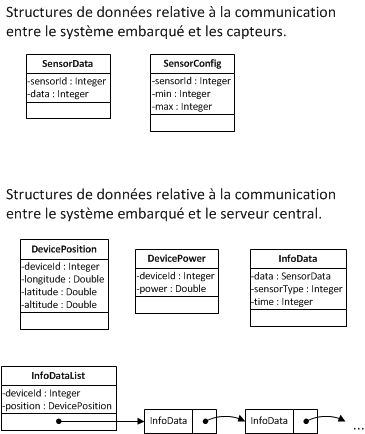
\includegraphics[width=8cm]{\PIXPATH/donnees2}
    \end{figure}
